\documentclass{beamer}

\newenvironment{tightcenter}{%
  \setlength\topsep{0pt}
  \setlength\parskip{0pt}
  \begin{center}
}{%
  \end{center}
}

\newenvironment{Snippet}{\Verbatim[samepage=true,fontsize=\tiny]}{\endVerbatim}

\mode<presentation>
{
  \usetheme{Copenhagen}
  %%\usecolortheme[RGB={173,222,25}]{structure}
  \usecolortheme[RGB={255,0,0}]{structure}
  \setbeamertemplate{items}[circle]
  \setbeamercovered{transparent}
}

\usepackage[polish]{babel}
\usepackage{chessfss}
\usepackage{hyperref}
\usepackage{qtree}
\usepackage{mathtools}
\usepackage{dirtytalk}
\usepackage{epigraph}
\usepackage{textgreek}
\usepackage[utf8]{inputenc}
\usepackage{times}
\usepackage[T1]{fontenc}
\usepackage{tikz}
\usepackage{csquotes}
\usepackage{amsmath}
\usepackage{fancyvrb}
\usepackage{ulem}
\usepackage{adjustbox}

\newcommand{\pawnB}[1][1.3ex]{%
  \adjustbox{Trim=4.3pt 2.6pt 4.3pt 0pt,width=#1,margin=0.2ex 0ex 0.2ex 0ex}{\BlackPawnOnWhite}%
}%
\newcommand{\rookB}[1][1.58ex]{%
  \adjustbox{Trim=3.2pt 2.2pt 3.2pt 0pt,width=#1,raise=0ex,margin=0.1ex 0ex 0.1ex 0ex}{\BlackRookOnWhite}%
}%
\newcommand{\knightB}[1][1.85ex]{%
  \adjustbox{Trim=2.3pt 2.35pt 2.5pt 0pt,width=#1,raise=-0.03ex,margin=0.14ex 0ex 0.14ex 0ex}{\BlackKnightOnWhite}%
}%
\newcommand{\bishopB}[1][1.79ex]{%
  \adjustbox{Trim=2.3pt 2pt 2.3pt 0pt,width=#1,raise=-0.12ex,margin=0.1ex 0ex 0.1ex 0ex}{\BlackBishopOnWhite}%
}%
\newcommand{\queenB}[1][2.05ex]{%
  \adjustbox{Trim=1.2pt 2.2pt 1.2pt 0pt,width=#1,raise=-0.08ex,margin=0.1ex 0ex 0.1ex 0ex}{\BlackQueenOnWhite}%
}%
\newcommand{\kingB}[1][1.95ex]{%
  \adjustbox{Trim=2pt 2pt 2pt 0pt,width=#1,raise=-0.06ex,margin=0.13ex 0ex 0.13ex 0ex}{\BlackKingOnWhite}%
  }%

\title{\textbf{The Culture of Scheme Programming}}

\author{Panicz Maciej Godek}

\institute{
  \tiny{\href{mailto:godek.maciek@gmail.com}{\textbf{godek.maciek@gmail.com}}}
}

\date{\textbf{Functional Tricity\#2}, 30.06.2016}

\begin{document}

\begin{frame}
  \titlepage
\end{frame}

\section{Introduction}

\subsection{What is a computer program?}

\begin{frame}{What is a computer program?}

  \textbf{What is a computer program?}
  \pause
  \begin{itemize}
  \item
    a set of instructions for a computer to execute
    under some specified circumstances
  \end{itemize}
\end{frame}


\begin{frame}{Computer program as a set of instructions}

  \textbf{Implications:}
  \pause
  \begin{itemize}
  \item
    instruct computer how to perform a computation
    \pause
  \item
    if certain patterns repeat, extract them to separate procedures
      
  \end{itemize}
\end{frame}

{ % all template changes are local to this group.
  \setbeamertemplate{navigation symbols}{}
  \begin{frame}[plain]
    \begin{tikzpicture}[remember picture,overlay]
      \node[at=(current page.center)] {
        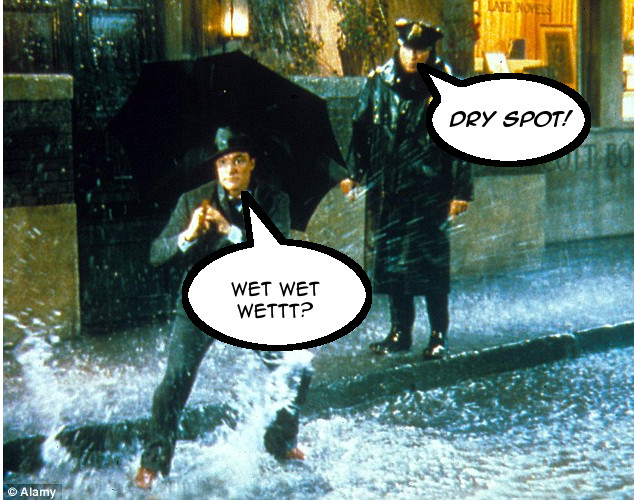
\includegraphics[width=\paperwidth,height=\paperheight]{dryspot.jpg}
      };
    \end{tikzpicture}
  \end{frame}
}

\begin{frame}{What is a computer program?}

  \textbf{What is a computer program?}
  \begin{itemize}
  \item
    a set of instructions for a computer to execute
    in some specified circumstances
    \pause
  \item
    a way of expressing ideas, communicating them to other people
  \end{itemize}
\end{frame}

\subsection{The anatomy of ideas}

\begin{frame}{The anatomy of ideas}

  \textbf{What is an idea?}
  \pause
  \begin{description}
  \item [idea] -- gr. \textiota\textdelta\textepsilon\textiota\textnu -- to see;
    \textepsilon\textiota\textdelta\textomikron\textvarsigma -- form, essence,
    type, species
  \end{description}
  \pause
  \textit{What can we do with ideas?}
  
\end{frame}

\begin{frame}{The anatomy of ideas}

  \begin{displayquote}
    The acts of the mind (...) are chiefly these three:
    \begin{enumerate}
    \item <2-> Combining several \textit{simple ideas} into one
      \textit{compound one}, and thus all \textbf{complex ideas} are made.
    \item <3-> (...) bringing two ideas, whether simple or complex, together,
      [...], without uniting them into one, by which it gets all its
      \textbf{ideas of relations}.
    \item <4-> (...) separating them from all other ideas that accompany them
      in their real existence: this is called abstraction, and thus all
      its \textbf{general ideas} are made.
    \end{enumerate}
  \end{displayquote}
  --- John Locke, \textit{An Essay Concerning Human Understanding} (1690)
  
\end{frame}

\begin{frame}{The anatomy of ideas}
  Inductive definition. An \textit{idea} is either:
  \begin{itemize}
    \pause
  \item one of the simple ideas
    \pause
  \item a complex idea -- a combination of simpler ideas
    \pause
  \item a general idea -- an abstraction over combinations of ideas
  \end{itemize}
\end{frame}


\begin{frame}{Understanding understanding}

  \textbf{What does it mean to understand an idea?}
  \begin{itemize}
    \pause
  \item reduce a complex idea to the simpler ones that can be considered
    obvious
    \pause
  \item being able to map the ideas onto our experience and imagination
    \pause
  \item being able to draw practical conclusions and apply the idea to
    one's own existential situation
  \end{itemize}

\end{frame}


\begin{frame}{Understanding understanding}

  \pause
  \begin{displayquote}
    Programming is understanding
  \end{displayquote}
  --- Kristen Nygaard

  \pause
  \begin{displayquote}
    You think you know when you can learn, are more sure when you can write,
    even more when you can teach, but certain when you can program.
  \end{displayquote}
  --- Alan Perlis
  
\end{frame}

\begin{frame}{Understanding understanding}
  
  \textbf{Why do we need ideas?}
  \pause
  
  \textbf{Why do we need complex ideas?}
  \pause

  \textbf{What are the means by which we create new ideas?}
  
\end{frame}


\begin{frame}{Definition of a definition}

  \begin{description}
    \item [definition] -- a linguistic expression whose purpose is to
    introduce a new term based on some terms that are already known.
  \end{description}
  
\end{frame}

\begin{frame}{Definition of a definition}

  \begin{description}
  \item [$\overbrace{\text{definition}}^{\text{definiendum}}$]
    -- $\overbrace{\text{a linguistic expression...}}^{\text{definiens}}$
  \end{description}
  
\end{frame}

\begin{frame}{Definition of a definition}

  \begin{description}
  \item [definition]
    -- $\overbrace{\text{a linguistic expression}}^{\text{genus}}
    \underbrace{\text{whose purpose...}}_{\text{differentia}}$
  \end{description}
  
\end{frame}

\begin{frame}{More sophisticated example}

  $M=\langle Q,\Gamma,\delta,q_{0},F\rangle,$
  where
  \begin{description}
  \item [$Q$] -- finite, non-empty set of states,
  \item [$\Gamma$] -- finite, non-empty set of \textit{alphabet symbols}
  \item [$\delta : Q\times\Gamma\mapsto Q\times\Gamma\times\{L,R\}$]
    -- state transition function
  \item [$q_{0}\in Q$] -- initial state
  \item [$F\subseteq Q$] -- a set of final states
  \end{description}
  
\end{frame}

\begin{frame}{Principle of compositionality}

  \textit{the meaning of a complex expression is determined by the meanings
  of its constituent expressions and the rules used to combine them}

  (Gottlob Frege)

  \pause
  \vspace{5mm}
  \textbf{Hypothesis:} in a complex expression, one can distinguish a ruling
  word which determines the meaning of the whole expression.
  
\end{frame}

\begin{frame}{Principle of compositionality}

  \textbf{Conclusion:} the structure of a compound expression (and its
  corresponding notion) can be represented as a tree.

  \pause
  \vspace{5mm}
  
  \Tree [.sum 
    [.squares 
      [.prime-numbers initial seven ] ] ]

  \textbf{Consequence:} Languages have syntactic (and semantic) structures.
  
\end{frame}

\subsection{Human and language}

\begin{frame}{Human and language}

  \textbf{Who we are?}

  \pause
  
  \textzeta\textomega\textomikron\textnu
  \ \textlambda\textomikron\textgamma\textomikron\textnu
  \ \textepsilon\textchi\textomega\textnu

  \pause
  
  \begin{displayquote}
    And out of the ground the LORD God formed every beast of the field,
    and every fowl of the air; and brought them unto Adam to see
    what he would \textit{call} them: and whatsoever Adam \textit{called}
    every living creature, that was the name thereof.
  \end{displayquote}
  --- Genesis 2:19
  
\end{frame}

\begin{frame}{Human and language}

  \textbf{How can we know?}

  \pause

  \begin{displayquote}
    The limits of my language mean the limits of my world.
  \end{displayquote}
  --- Ludwig Wittgenstein

  \pause

  \begin{displayquote}
    We dissect nature along lines laid down by our native language.
    The categories and types that we isolate from the world of phenomena
    we do not find there because they stare every observer in the face;
    on the contrary, the world is presented in a kaleidoscope flux
    of impressions which has to be organized by our minds—and this
    means largely by the linguistic systems of our minds.
  \end{displayquote}
  --- Benjamin Whorf
  
\end{frame}

\begin{frame}{What does it mean to mean?}


  \textbf{How is communication possible?}
  \begin{itemize}
    \pause
    
    \item \textiota\textdelta\textiota\textomikron\textvarsigma
      \ \textkappa\textomikron\textsigma\textmu\textomikron\textvarsigma \\*
      \pause
      \textit{“When I use a word,” Humpty Dumpty said, in rather a scornful tone,
        “it means just what I choose it to mean—neither more nor less.”}
      \\* --- Lewis Carroll, \textit{Through the Looking Glass}

      \pause
      
    \item \textkappa\textomikron\textiota\textnu\textomikron\textvarsigma
      \ \textkappa\textomikron\textsigma\textmu\textomikron\textvarsigma
    
  \end{itemize}
  
\end{frame}


\begin{frame}{How natural is natural language?}

  \textbf{How about using natural language to communicate ideas?}
  
\end{frame}


\begin{frame}{How natural is natural language?}

  Imprecision and ambiguity:
  \begin{itemize}
    \pause
  \item Iraqi Head Seeks Arms
    \pause
  \item Prostitutes Appeal to Pope
    \pause
  \item Soviet Virgin Lands Short of Goal Again
    \pause
  \item Regan Wins on Budget, but More Lies Ahead
  \end{itemize}
  
\end{frame}

\begin{frame}{How natural is natural language?}

  Complicated structure
  \pause
  \begin{displayquote}
    I suspect that machines to be programmed in our native tongues —be it Dutch,
    English, American, French, German, or Swahili— are as damned
    difficult to make as they would be to use.
  \end{displayquote}
  --- Edsger Dijkstra, \textit{On the Foolishness of ``Natural Language Programming''}
\end{frame}


\begin{frame}[fragile]{How natural is natural language?}
  
  \begin{Snippet}
    Hanoi is a room.
    
    A disk is a kind of supporter.
    
    A post is a kind of supporter. A post is always fixed in place.
    
    The left post, the middle post, and the right post are posts in Hanoi.
    
    A disk is a kind of supporter.
    The red disk is a disk on the left post.
    The orange disk is a disk on the red disk.
    The yellow disk is a disk on the orange disk.
    The green disk is a disk on the yellow disk.

    Definition: a disk is topmost if nothing is on it.

    When play begins:
        move 4 disks from the left post to the right post via the middle post.

    To move (N - number) disk/disks from (FP - post) to (TP - post) via (VP - post):
        if N > 0:
            move N - 1 disks from FP to VP via TP;
            say ``Moving a disk from [FP] to [TP]...'';
            let D be a random topmost disk enclosed by FP;
            if a topmost disk (called TD) is enclosed by TP, now D is on TD;
            otherwise now D is on TP;
            move N - 1 disks from VP to TP via FP.
  \end{Snippet}

\end{frame}

\begin{frame}{How natural is natural language?}

  Verbosity
  \pause
  \begin{displayquote}
    By relieving the brain of all unnecessary work, a good notation
    sets it free to concentrate on more advanced problems, and
    in effect increases the mental power of the race.
  \end{displayquote}
  --- Alfred N. Whitehead, \textit{An Introduction to Mathematics}
  \pause
  \begin{small}
  \begin{displayquote}
    In the twelfth century, the Hindu mathematician Bhaskara said,
    ``The root of the root of the quotient of the greater irrational
    divided by the lesser one being increased by one; the sum being
    squared and multiplied by the smaller irrational quantity is the
    sum of the two surd roots.''
    \pause
    $\sqrt{(\sqrt{\frac{n}{k}}+1)^{2}k}=\sqrt{k}+\sqrt{n}$
  \end{displayquote}
  \end{small}
  --- Gilles Fauconner, Mark Turner, \textit{The Way We Think}
  
\end{frame}

\begin{frame}{Is mathematics the language of nature?}
  \textbf{How about using mathematics to express ideas?}
  \begin{itemize}
    \pause
  \item compact notation
    \pause
  \item ``algebra of programs''
    \pause
  \item funny symbols (Uncle Bob wouldn't like it)
  \end{itemize}
\end{frame}

\subsection{Advantages of functional programming}

\begin{frame}{Why functional programming?}

  \textbf{What is so great about functional programming?}  
  \begin{itemize}
    \pause
  \item easier to reason about
    \pause
  \item no type errors
    \pause
  \item referential transparency
    \pause
  \item ...
    \pause
  \item no side effects
  \end{itemize}
  
\end{frame}

{ % all template changes are local to this group.
  \setbeamertemplate{navigation symbols}{}
  \begin{frame}[plain]
    \begin{tikzpicture}[remember picture,overlay]
      \node[at=(current page.center)] {
        
\includegraphics[height=\paperheight]{condoms.jpg}
      };
    \end{tikzpicture}
  \end{frame}
}

\begin{frame}{Why functional programming?}

  \begin{displayquote}
    In the beginning was the Word, and the Word was with God,
    and the Word was God.
  \end{displayquote}
  --- John 1:1
  \pause
  \begin{itemize}
  \item substitution model of computation (conotation)
    \pause
  \item program is just a name of some compound object (denotation)
  \end{itemize}
  \pause
  \textbf{Functional programming is like speaking language}
  
\end{frame}

\begin{frame}{Intermission}
  \begin{center}
    \begin{Huge}
      And now...
    \end{Huge}
  \end{center}
\end{frame}

\begin{frame}{Intermission}

  \begin{displayquote}
    I hope the field of computer science never loses its sense of fun. Above all,
    I hope we don't become missionaries. Don't feel as if you're Bible salesmen.
    The world has too many of those already. 
  \end{displayquote}
  --- Alan Perlis, foreword to \textit{Structure and Interpretation of Computer Programs}
\end{frame}

\begin{frame}{The philosophy of Scheme}
  \begin{center}
    \begin{Huge}
      The Culture of Scheme Programming
    \end{Huge}
  \end{center}
  
\end{frame}

\section{The philosophy of Scheme}

\begin{frame}{The philosophy of Scheme}
  \begin{displayquote}
    Perfection is finally attained not when there is no longer
    anything to add, but when there is no longer anything to take away.
  \end{displayquote}
  ---  Antoine de Saint-Exupery
  \pause
  \begin{displayquote}
    Programming languages should be designed not by piling feature
    on top of feature, but by removing the weaknesses and restrictions
    that make additional features appear necessary.
  \end{displayquote}
  --- Revised$^5$ Report on the Algorithmic Language Scheme
  \pause
  \textbf{What are the necessary components of an expressive programming language?}
  
\end{frame}

\subsection{Syntax}

\begin{frame}{The syntax of Scheme}

  Recall the Principle of Compositionality:
  \pause
  \begin{displayquote}
    the meaning of a complex expression is determined by the meanings
    of its constituent expressions and the rules used to combine them
  \end{displayquote}
  \pause
  Apply the following conventions:
  \begin{itemize}
    \pause
  \item write the ruling word (or the name of the combining rule) as the first
    element
    \pause
  \item write the constituent expressions to the right of the ruling word;
    the order in which they are written determines their role in a given rule
    \pause
  \item surround the combination in parentheses
    \pause
  \item \textit{et voila!}
  \end{itemize}
  
\end{frame}

\begin{frame}{The syntax of Scheme}
  ``Sum of squares of initial seven prime numbers'' \\*
  \pause
  \Tree [.sum 
    [.squares 
      [.prime-numbers initial seven ] ] ]
  \\*
  \pause
  \texttt{(sum (squares (prime-numbers initial seven)))}
  \pause
  Note: the latter is more versatile!
\end{frame}

\begin{frame}{The syntax of Scheme}

  \textbf{A Quiz: which syntax is better?}
  
  \begin{columns}[T] % align columns
    \begin{column}{.48\textwidth}
      %\rule{\linewidth}{4pt}
      \begin{small}
        \texttt{int factorial(int n) \{\\*
            \ \ int result = 1;\\*
            \ \ for (int i = 1; i <= n; ++i)\\*
            \ \ \ \ result *= i;\\*
            \ \ return result;\\*
            \}}
      \end{small}
    \end{column}%
    \hfill%
    \begin{column}{.48\textwidth}
      \begin{small}
        \texttt{function factorial(n: integer): integer;\\*
          \ var\\*
          \ \ i, result: integer;\\*
          \ begin\\*
          \ \ result := 1;\\*
          \ \ for i := 2 to n do\\*
          \ \ \ result := result * i;\\*
          \ \ factorial := result\\*
          \ end;}
       \end{small}
    \end{column}%
  \end{columns}  
\end{frame}


\begin{frame}{The syntax of Scheme}
  \begin{center}
    \huge{Homoiconicity}
  \end{center}
\end{frame}

\begin{frame}{The syntax of Scheme}
  \begin{center}
    \huge{Homoiconicity}\\*
    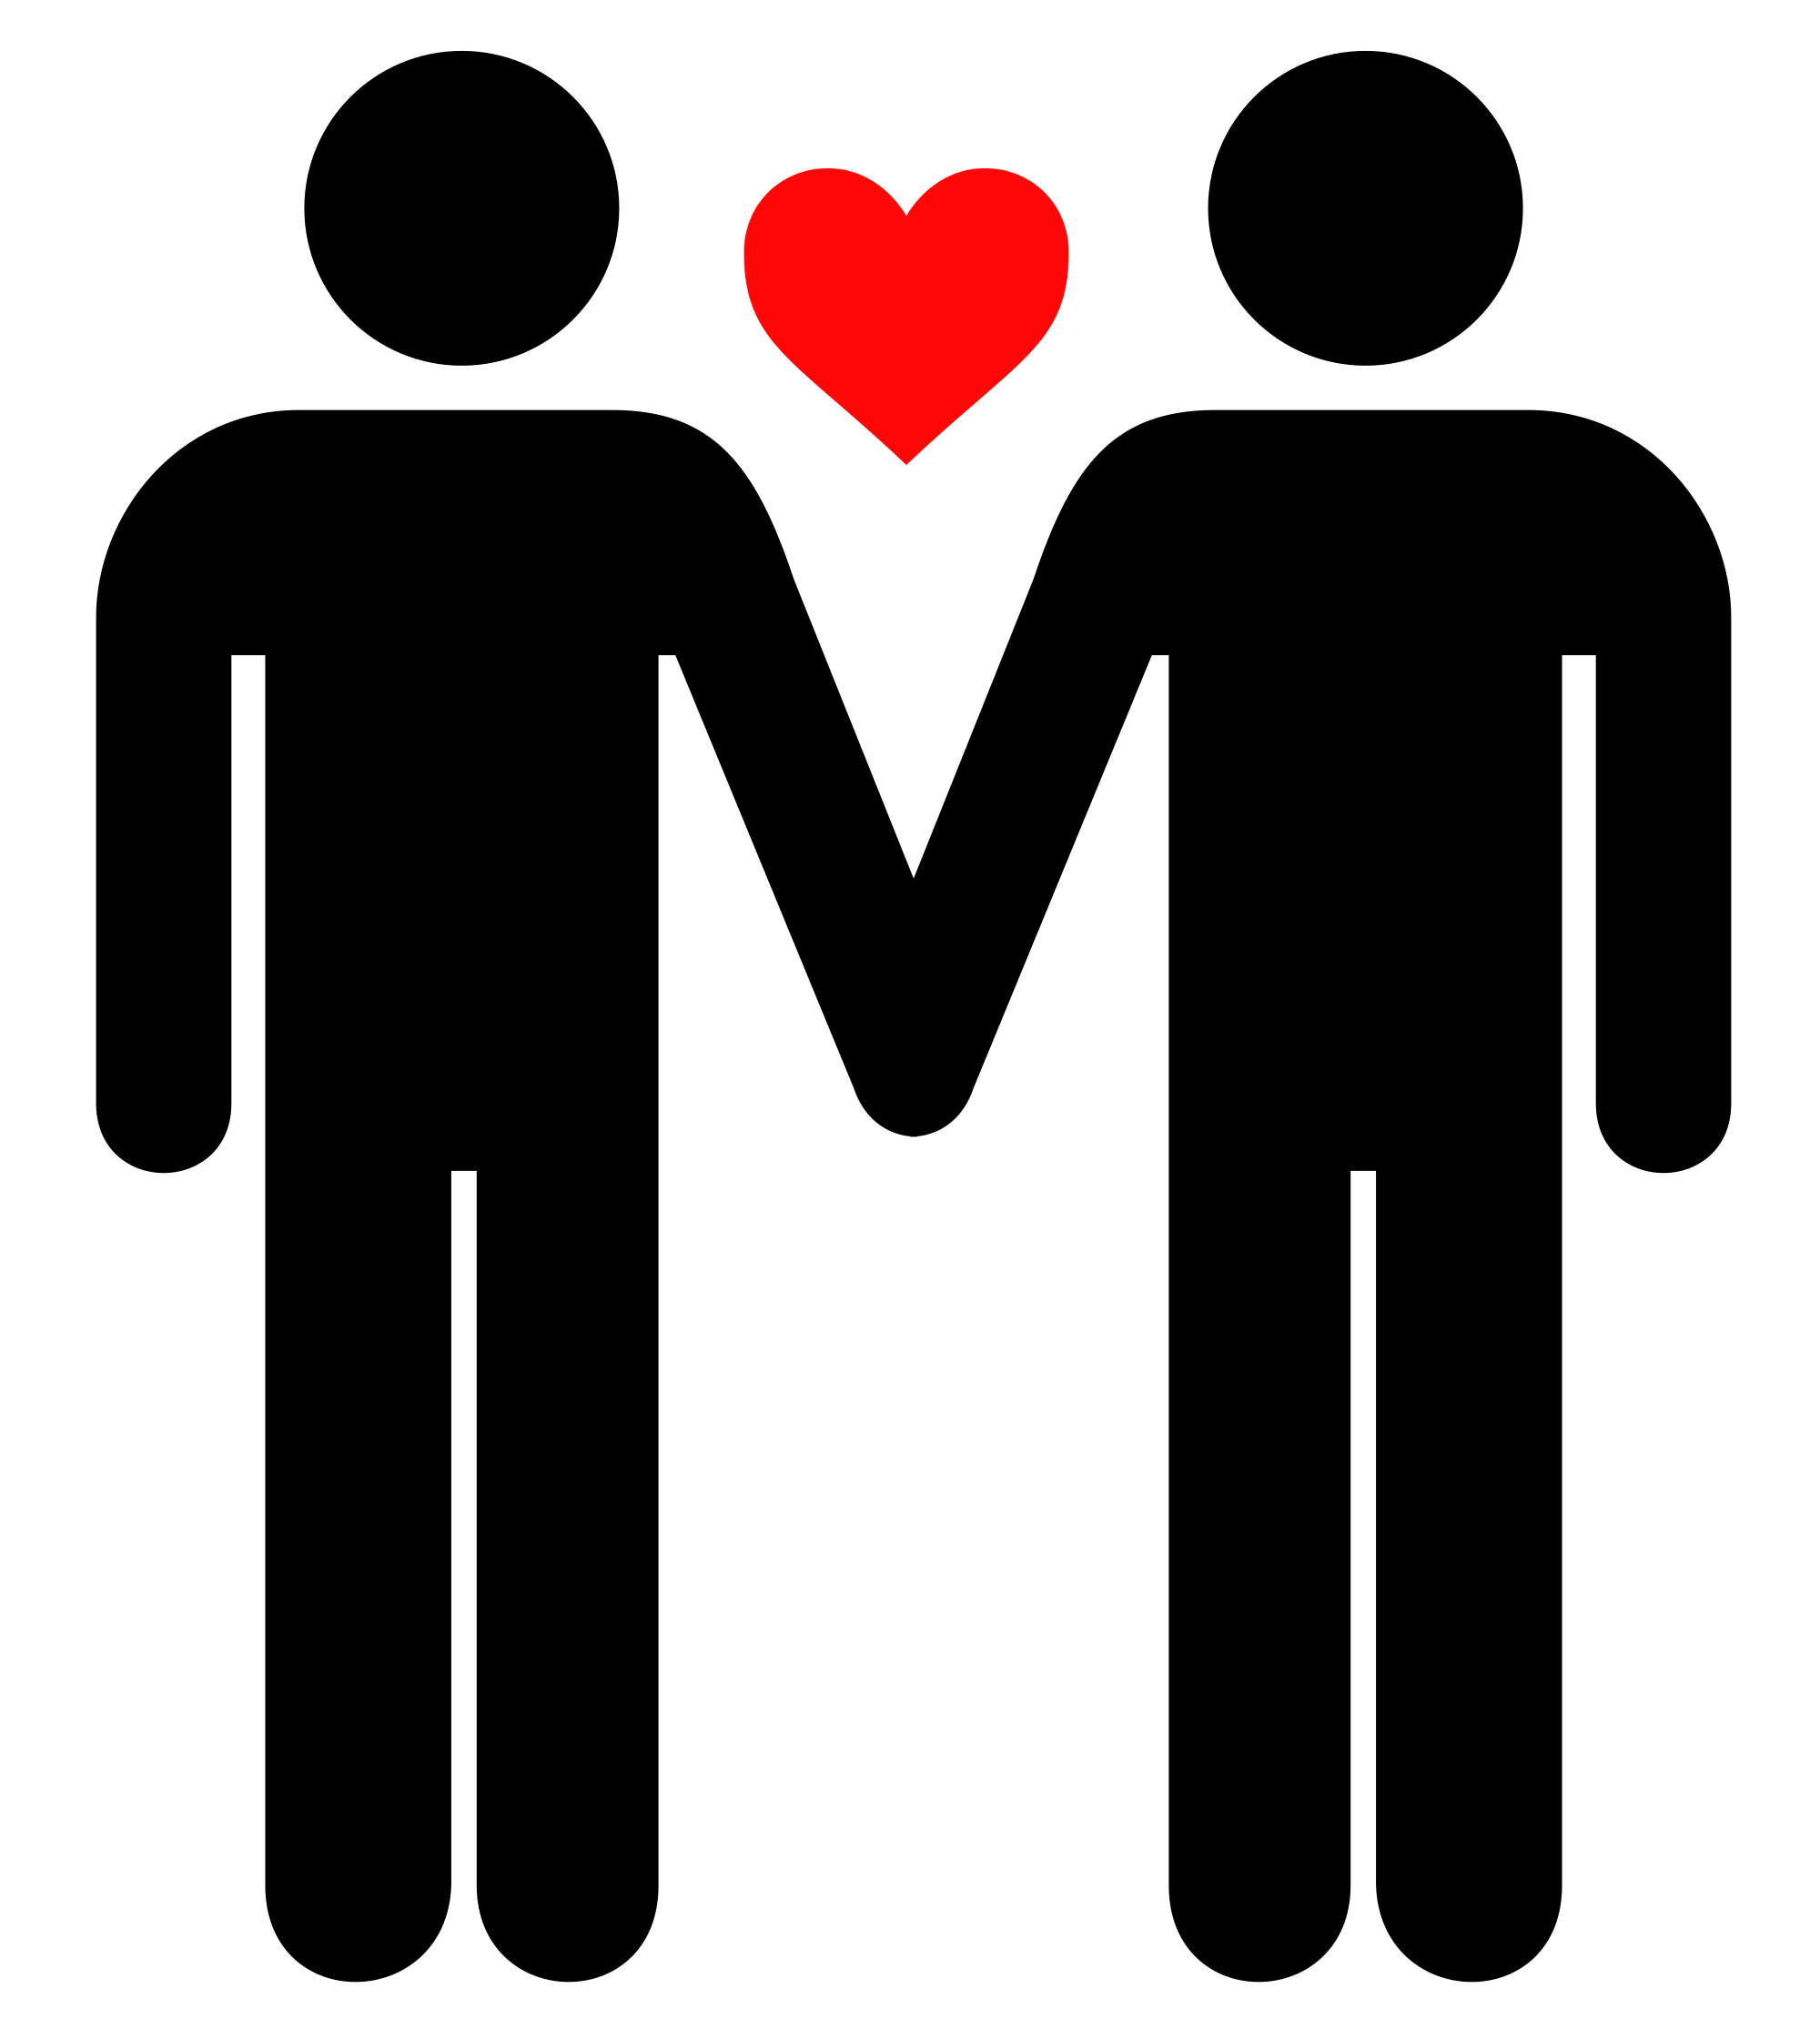
\includegraphics[width=0.4\textwidth]{homoiconic.png}\\*
  \end{center}
\end{frame}

\subsection{Semantics}

\begin{frame}{The semantics of Scheme}
  \center{\huge{\textlambda-calculus}}
  \begin{itemize}
    \pause
  \item substitution model of computation \\*
    \pause $\lambda x . \text{\textbf{This is }} x \text{\textbf{!}}$ \\*
    \pause $(\lambda x . \text{\textbf{This is }} x \text{\textbf{!}})
    \text{\textbf{it}}$ \\*
    \pause $\Rightarrow \text{\textbf{This is it!}}$ \pause
  \item lexical scoping, applicative order of evaluation
  \end{itemize}
\end{frame}

\begin{frame}{The semantics of Scheme}
  \textbf{Special forms:}
  \begin{itemize}
    \pause
  \item \texttt{(\textbf{define} \textit{definiendum} \textit{definiens})}
    \pause
  \item \texttt{(\textbf{lambda} (\textit{arguments ...}) \textit{body})}
    \pause
  \item \texttt{(\textbf{if} \textit{then} \textit{else})}
    \pause
  \item \texttt{(\textbf{quote} \textit{s-exp})}
    \pause
  \item \texttt{(\textbf{set!} \textit{variable} \textit{value})}
    \pause
  \item \texttt{(\textbf{begin} \textit{expression ...})}
  \end{itemize}
\end{frame}


\begin{frame}{The semantics of Scheme}
  \textbf{Control structures:}
  \texttt{
    \begin{itemize}
      \pause
    \item goto
      \pause
    \item break
      \pause
    \item continue
      \pause
    \item return
      \pause
    \item throw/catch
      \pause
    \item yield
    \end{itemize}
  }
\end{frame}

\begin{frame}{The semantics of Scheme}
  \textbf{Control structures:}
  \texttt{
    \begin{itemize}
    \item \sout{goto}
    \item \sout{break}
    \item \sout{continue}
    \item \sout{return}
    \item \sout{throw/catch}
    \item \sout{yield}
    \item call-with-current-continuation
    \end{itemize}
  }
\end{frame}

\begin{frame}{The semantics of Scheme}
  \textbf{Self-describability:}
  \pause
  \begin{displayquote}
    The evaluator, which determines the meaning of expressions
    in a programming language, is just another program.
  \end{displayquote}
  --- the most fundamental idea in programming
\end{frame}

\subsection{Conventions}

\begin{frame}{The conventions of Scheme}
  \textbf{A Quiz: which notation is better?}
  \vspace{15mm}
  \begin{columns}[T]
    \begin{column}{.48\textwidth}
      \texttt{under\_score\_notation}
    \end{column}
    \hfill
    \begin{column}{.48\textwidth}
      \texttt{camelCaseNotation}
    \end{column}
  \end{columns}
  \pause
  \center{\texttt{why-even-bother?}}
\end{frame}

\begin{frame}[fragile]{The conventions of Scheme}
  \textbf{Minimal number of rules?}
  \begin{Verbatim}
    K(SII(S(K(S(S(KS)
    (S(K(S(KS)))
    (S(K(S(KK)))
    (S(K(S(K(S(K(S(K(S(SI(K(S(K(S(S(KS)K)I))
    (S(S(KS)K)(SII(S(S(KS)K)I))))))))K))))))
    (S(K(S(K(S(SI(K(S(K(S(SI(K(S(K(S(S(KS)K)I))
    (S(S(KS)K)(SII(S(S(KS)K)I))
    (S(S(KS)K))(S(SII)I(S(S(KS)K)I))))))))
    K)))))))
    (S(S(KS)K)(K(S(S(KS)K)))))))))
    (K(S(K(S(S(KS)K)))K))))(SII))II)
  \end{Verbatim}
\end{frame}

\section{The Crops}

\begin{frame}{Learnable}
  The story of 7 year old Zora Ball: \\*
  \url{https://www.youtube.com/watch?v=9oEZjpEqCwM}
\end{frame}

\begin{frame}{Easy to implement}
  \textbf{Multitude of implementations:}
  \begin{itemize}
    \pause
  \item Chez
    \pause
  \item Racket
    \pause
  \item Kawa
    \pause
  \item Gambit (+termite)
    \pause
  \item Guile
    \pause
  \item Biwa
    \pause
  \item Iron Scheme
    \pause
  \item ... and more (approx. 80): \url{http://www.schemers.org/Implementations/}
  \end{itemize}
\end{frame}

\begin{frame}[fragile]{Managable}
  \textbf{Easy to manipulate syntax tree}
  \begin{itemize}
  \item <1-> syntax transformers (macros)\\*
    \texttt{\uncover<2->{(define-syntax} (let ((name value) ...)\\*
      \ \ \ \ \ \ \ \ \ \ \ \ \ \ \ \ \ \ body . *)\\*
      \ \ ((lambda (name ...) body . *) value)\uncover<2->{)} }
  \item <3-> single-expression comments\\*
    \texttt{(i can \uncover<4->{\#;(comment out (nested) expressions!)} and you?)}
  \item <5-> possible to evaluate single expressions on the fly (e.g. geiser)
  \end{itemize}
\end{frame}

\begin{frame}{Fixable}
  \textbf{Possible to override core bindings}
  \begin{itemize}
    \pause
  \item curried definitions\\*
    {\small \texttt{(define ((f x) y) body)\\*
        === (define f (lambda (y) (lambda (x) body)))}}
    \pause
    \item pattern-matching lambdas\\*
    \texttt{(lambda ((x . y)) x) === car}
  \end{itemize}
\end{frame}

\begin{frame}{Original ideas}
  \textbf{Some ideas unthinkable in other languages:}
  \begin{itemize}
    \pause
  \item running evaluator backwards: \url{https://www.youtube.com/watch?v=eQL48qYDwp4}
    \pause
  \item ferns/engines \url{http://projects.csail.mit.edu/wiki/pub/JoeNear/FernMonad/frons.pdf}
    \pause
  \item lazy streams (``Cons Should Not Evaluate Its Arguments'')
  \end{itemize}
\end{frame}

\section{Showcase/Controversies/Books}
\begin{frame}[fragile]{What does the ``of'' mean?}
  \textbf{How do you memoize the order of arguments to a function?}
  \pause
  \begin{Snippet}
(define (shortest-cycle #;from first . #;through rest)

  (define (shortest-path #;from node #;to target #;through nodes)
    (if (null? nodes)
      `((,node ,target) ,(distance #;from node #;to target))
       (let* ((subpaths (map (lambda (node)
                               (let ((other-nodes (delete node #;from nodes)))
                                 (shortest-path #;from node #;to target
                                              #;through other-nodes)))
                             nodes))
              ((path _) increased-cost
                        (argmin (λ (((next . _) cost))
                                  (+ cost (distance #;from node #;to next)))
                                subpaths)))
         `((,node . ,path) ,increased-cost))))

  (apply values (shortest-path #;from first #;to first #;through rest)))
  \end{Snippet}
\end{frame}

\begin{frame}[fragile]{Showing and telling}
  \begin{displayquote}
    Better explain than instruct; better show than tell
  \end{displayquote}
  \pause
  \texttt{(define-chess-rules\\*
    \ \ (initial-board:\\*
    \ \ \ ((\rookB\ \pawnB\ \_ \_ \_ \_ \pawn\ \rook)\\*
    \ \ \ \ (\knightB\ \pawnB\ \_ \_ \_ \_ \pawn\ \knight)\\*
    \ \ \ \ (\bishopB\ \pawnB\ \_ \_ \_ \_ \pawn\ \bishop)\\*
    \ \ \ \ (\kingB\ \pawnB\ \_ \_ \_ \_ \pawn\ \king)\\*
    \ \ \ \ (\queenB\ \pawnB\ \_ \_ \_ \_ \pawn\ \queen)\\*
    \ \ \ \ (\bishopB\ \pawnB\ \_ \_ \_ \_ \pawn\ \bishop)\\*
    \ \ \ \ (\knightB\ \pawnB\ \_ \_ \_ \_ \pawn\ \knight)\\*
    \ \ \ \ (\rookB\ \pawnB\ \_ \_ \_ \_ \pawn\ \rook))\\*
    ...}
\end{frame}


\begin{frame}[fragile]{Showing and telling}
  \texttt{...\\*
    \ \ (\bishopB\\*
    %\ \ \ (((\queenB\ \_\ $\rightarrow$\ $\square$/\_))\\*
    %\ \ \ \ ;;==========\\*
    %\ \ \ \ ((\_\ \_\ $\rightarrow$\ \ \queenB))\\*
    \ \ \ (((?\ ?\ $\cdots$\ $\square$/\_)\\*
    \ \ \ \ \ ($\vdots$\ $\vdots$\ $\nearrow$\ \ $\vdots$)\\*
    \ \ \ \ \ (?\ \_\ $\cdots$\ ?)\\*
    \ \ \ \ \ (\bishopB\ ?\ $\cdots$\ ?))\\*
    \ \ \ \ ;;==========\\*
    \ \ \ \ ((?\ ?\ $\cdots$\ \bishopB)\\*
    \ \ \ \ \ ($\vdots$\ $\vdots$\ $\nearrow$\ \ $\vdots$)\\*
    \ \ \ \ \ (?\ \_\ $\cdots$\ ?)\\*
    \ \ \ \ \ (\_\ ?\ $\cdots$\ ?))\\*
    \ \ \ \ (symmetries: all-rotations))\\*
    ...
  }
\end{frame}


\begin{frame}[fragile]{Showing and telling}
  \textbf{What does the following code do?}
  \pause
  \begin{Verbatim}
(define (upper-left-corner rect w h)
  (map (lambda (row)
         (take row w))
    (take rect h)))
  \end{Verbatim}
  \pause
  \begin{Verbatim}
(e.g. (upper-left-corner '((a b c d)
                           (e f g h)
                           (i j k l)) 3 2)
    ===> ((a b c)
          (e f g)))
  \end{Verbatim}
\end{frame}

\begin{frame}[fragile]{Showing and telling}
  \textbf{Is the purity really that important?}
  \begin{Verbatim}
(define (cross-over daddy mommy)
  (assert (= (length daddy) (length mommy)))
  (let* ((position (random (length daddy)))
	 (sperm (take daddy position))
	 (ovum (drop mommy position)))
    `(,@sperm ,@ovum)))
  \end{Verbatim}
\end{frame}


\begin{frame}{Controversies (and responses)}

  \textbf{Criticism:}
  \begin{itemize}
    \pause
  \item Lots of Irritating Superfluous Parentheses!
    \pause
  \item Phil Wadler, ``Why Calculating is Better Than Scheming''
    \begin{itemize}
      \pause
    \item no pattern matching
      \pause
    \item unfamiliar syntax
      \pause
    \item no types
      \pause
    \item no lazy evaluation
    \end{itemize}
    \pause
  \item ungooglable name
    \pause
  \item no libraries
    \pause
  \item R6RS controversy
  \end{itemize}
    
\end{frame}

\begin{frame}{Controversies (and responses)}
  \textbf{The newcomer's perspective}
  \begin{displayquote}
    Why is it that you consider the R5RS the last ``true'' Scheme? (...)

    Is it a particular feature set?  A limit on page count?
    Utter minimalism to the point of being virtually useless without
    implementation-dependent extensions?  What? (...)

    It seems to me that many Schemers have some ideal in their minds about
    what Scheme *really* is, but that language is imaginary, existing only
    in the R5RS document. (...)
  \end{displayquote}
  --- Internet user, comp.lang.scheme
\end{frame}


\begin{frame}{Controversies (and responses)}
  \begin{displayquote}
    Scheme would still be useful as a notation for expressing
    computational methods even in the absence of a mechanical
    implementation.
  \end{displayquote}
  --- Revised$^5$ Report on the Algorithmic Language Scheme
\end{frame}

\begin{frame}{Important books}
  \textbf{Books:}
  \begin{itemize}
    \pause
  \item Hal Abelson, Gerald Sussman, ``Structure and Interpretation of Computer Programs'', \url{https://mitpress.mit.edu/sicp/}
    \pause
  \item Daniel Friedman, Mitchell Wand, ``Essentials of Programming Languages'', \url{http://www.eopl3.com/}
    \pause
  \item Mathias Felleisen, Robert Findler, Matthew Flat, Shiram Krishnamurthi, ``How to Design Programs'', \url{http://www.htdp.org/}
    \pause
  \item Daniel Friedman et al., ``The Little Schemer'', ``The Seasoned Schemer'',  ``The Reasoned Schemer'', ``The Little Prover''
  \end{itemize}
\end{frame}

\begin{frame}{Unimportant books}
  \textbf{Books -- continued:}
  \begin{itemize}
    \pause
  \item Panicz Maciej Godek, ``A Pamphlet Against R'', \url{http://panicz.github.io/pamphlet}
  \end{itemize}
\end{frame}

\begin{frame}{Ads}
  \begin{center}
    \huge{\url{http://roomofplenty.pl/}}\\*
    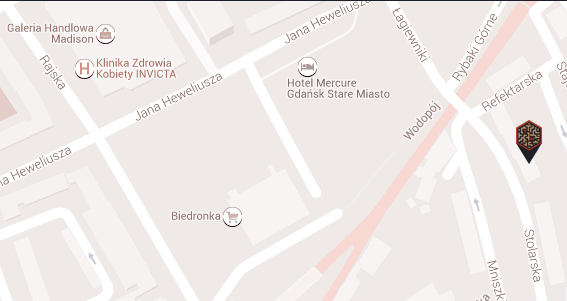
\includegraphics[width=0.8\textwidth]{plenty.png}\\*
  \end{center}
\end{frame}

\begin{frame}{The End}
  \begin{center}
    \huge{Questions?}\\%
    \normalsize{\href{mailto:godek.maciek@gmail.com}{godek.maciek@gmail.com}}\\*
    \normalsize{@PaniczGodek}
  \end{center}
\end{frame}


\end{document}
